\documentclass[12pt, a4paper]{book}

\usepackage{libertine}
\usepackage{libertinust1math}
\usepackage{inconsolata}
\usepackage{amsthm, amsmath}
\usepackage[style=german]{csquotes}
\usepackage[pagestyles]{titlesec}
\usepackage[romanian]{babel}
\usepackage{tikz}
\usetikzlibrary{er,positioning}
\usepackage{soul}
\usepackage{tocloft}
\usepackage{enumerate}
\usepackage{setspace}
\usepackage{subcaption}
\usepackage{bm}
\usepackage{xcolor}
\usepackage{todonotes}
\usepackage{graphicx}
\usepackage{array}
\usepackage[all]{xy}
\setcounter{MaxMatrixCols}{20}
\usepackage{fancyhdr}
% \usepackage{natbib}     % citekey hyphenation
\usepackage{marginnote}
\usepackage{imakeidx}
\makeindex[options= -s indices-alph.ist]
\usepackage{hyperref}
\hypersetup{citecolor=blue}
\usepackage{fontawesome}

\newcommand\NN{\mathbb{N}}
\newcommand\ZZ{\mathbb{Z}}
\newcommand\QQ{\mathbb{Q}}
\newcommand\RR{\mathbb{R}}
\newcommand\CC{\mathbb{C}}
\newcommand\AF{\mathbb{A}}
\newcommand\PP{\mathbb{P}}
\newcommand\FF{\mathbb{F}}
\newcommand\bb{\mathbb}
\newcommand\dr{\mathrm}
\newcommand\kal{\mathscr}
\newcommand\fk{\mathfrak}
\newcommand\op{\oplus}
\newcommand\ot{\otimes}
\newcommand\ds{\displaystyle}
\newcommand\id{\indent}
\newcommand\nid{\noindent}
\newcommand\seq{\subseteq}
\newcommand\sneq{\subsetneq}
\newcommand\speq{\supseteq}
\newcommand\spneq{\supsetneq}
\newcommand\rar{\rightarrow}
\newcommand\Rar{\Rightarrow}
\newcommand\xrar{\xrightarrow}
\newcommand\lar{\leftarrow}
\newcommand\Lar{\Leftarrow}
\newcommand\xlar{\xleftarrow}
\newcommand\lrar{\leftrightarrow}
\newcommand\Lrar{\Leftrightarrow}
\newcommand\ideal{\trianglelefteq}
\newcommand\such{\text{ s.t. }}
\newcommand\sk{(\textit{Sketch}) }
\newcommand\rhup{\rightharpoonup}
\newcommand\rhdn{\rightharpoondown}
\newcommand\lhup{\leftharpoonup}
\newcommand\lhdn{\leftharpoondown}
\newcommand\incl{\hookrightarrow}
\newcommand\vid{\emptyset}
\newcommand\wt{\widetilde}
\newcommand\wh{\widehat}
\newcommand\ol{\overline}
\newcommand\Lor{\Longrightarrow}
\newcommand\Lol{\Longleftarrow}
\newcommand\Lolr{\Longleftrightarrow}
\newcommand\ld{{}^\ast}
\newcommand\lgr{{}^{\ast-\text{gr}}}
\newcommand\kap{\Bbbk^a[\kal{P}]}
\newcommand\kcp{\Bbbk^c[\kal{P}]}
\newcommand\fc{\mathfrak{c}}
\newcommand\qq{\enquote}
\newcommand\coli{\protect\varinjlim}
\newcommand\li{\protect\varprojlim}
\newcommand\injr{\rightarrowtail}
\newcommand\surjr{\twoheadrightarrow}
\newcommand\injl{\leftarrowtail}
\newcommand\surjl{\twoheadleftarrow}
\newcommand\sqsb{\sqsubseteq}
% FONTS
\usepackage[mathscr]{euscript}
\usepackage[normalem]{ulem}
\usepackage{eurosym}
\usepackage{sectsty}
\allsectionsfont{\rmfamily}
\usepackage{anyfontsize}

% PAGE SETUP
\usepackage[portrait]{geometry}
\geometry{
  a4paper,
  left=20mm,
  right=25mm,
  % marginparwidth=40mm,
}
\usepackage{afterpage}
\newcommand\blankpage{
  \null
  \thispagestyle{empty}
  \addtocounter{page}{-1}
  \newpage}
\newenvironment{myenv}[1]
  {\begin{spacing}{#1}}
    {\end{spacing}}

% FANCY SETUP
\usepackage[Glenn]{fncychap}
\usepackage{fancyhdr}
\addto\captionsromanian{\renewcommand{\chaptername}{Secțiunea}}


\begin{document}

\thispagestyle{empty}
\pagestyle{plain} % fix for page numbers

\title{\Huge The Onion Router (\texttt{Tor})}
\vspace{1cm}
\author{\large\textsc{Cornel Bucurescu} \\
  \large\textsc{Adrian Manea} \\
\large\textsc{Cristian Nicolae}}

\maketitle

\pagenumbering{gobble}
\tableofcontents

\setcounter{page}{1} % page 1 after TOC

%%%%%%%%%%%%%%%%%%%%%%%%%%%%%%%%%%%%%%%%%%%%%%%%%%%%%%%%%%%%%%%%%%%%%%
% MAIN CONTENT
\addcontentsline{toc}{chapter}{\protect\numberline{}De ad\u{a}ugat sau clarificat}
\listoftodos[De ad\u{a}ugat sau clarificat]
\pagenumbering{arabic}

%! TEX root = ../tor.tex

\chapter{Generalități}

\section{Idei principale}

\indent\indent \qq{Rutarea în foi de ceapă} (eng.\ \textit{onion routing}, OR) a fost
concepută pentru anonimizarea aplicațiilor care funcționează pe baza protocolului
TCP, precum browsere, servicii de mesagerie sau \texttt{ssh}. În acest model
de rutare, clienții aleg un drum prin rețea, construind un circuit, dar
astfel încît fiecare nod cunoaște doar predecesorul și succesorul său, fără restul
nodurilor care ar putea exista în rețea.
\index{onion!routing (OR)}

Traficul propriu-zis criculă în pachete de mărime fixată, numite \emph{celule},
\index{celule} care sînt decodate cu o cheie simetrică în fiecare nod, apoi
transmise mai departe.

După înființarea proiectului, a apărut destul de repede o rețea de astfel de
noduri, dar chiar și la început, atunci cînd singurul nod era doar o mașină de teste,
procesa conexiuni de la peste 60 000 IP-uri din întreaga lume, cu un flux de
aproximativ 50 000 conexiuni pe zi.

Tor a fost conceput pentru a rezolva deficiențele găsite în modelul inițial OR,
iar principalele îmbunătățiri privesc:
\begin{enumerate}[(1)]
  \item \textit{Secretizarea perfectă a înaintării traficului} (eng.\ perfect
    forward secrecy): în modelul inițial, dacă exista un nod ostil într-un punct
    al conexiunii, putea să refuze înaintarea traficului și să decripteze
    conținutul care a ajuns pînă la el. În modelul actual, se folosește o
    \emph{criptare telescopică}, prin care nodul curent adaugă chei
    de sesiune la criptarea de pînă atunci și totodată pierde accesul la cheile din
    urmă, astfel încît mesajul să nu mai poată fi decriptat (nodul curent are
    acces doar la ultima parte a cheii, cu care contribuie).
    \index{criptare!telescopică}
  \item \textit{Separarea \qq{curățirii protocolului} de anonimitate:} în varianta
    inițială, OR cerea proxy-uri pentru aplicații, corespunzătoare fiecărei
    aplicații suportate. Dacă proxy-urile nu erau scrise (fiind un proces laborios),
    protocoalele suportau doar puține aplicații. Tor folosește o interfață
    proxy standard, SOCKS și proxy-uri de filtrare pentru aplicații de tip
    Privoxy, care sînt bine cunoscute și dezvoltate.
    \todo[inline,noline,backgroundcolor=green!40]{citări pentru SOCKS și Privoxy}
  \item \textit{Nu influențează traficul}: OR cerea gruparea și reordonarea
    celulelor care ajungeau la norduri și adăugarea de padding între utilizatori
    și OR-uri. \todo[inline,noline,backgroundcolor=green!40]{padding?}
    Această prelucrare suplimentară cerea standardizarea și găsirea unor algoritmi
    care să facă operațiunile sigure --- algoritmi care încă nu s-au găsit. Pînă
    la găsirea unor implementări satisfăcătoare, Tor nu \qq{modelează} în niciun
    fel traficul.
  \item \textit{Mai multe fire TCP pot folosi același circuit}: în implementarea
    originală, OR cerea construirea cîte unui circuit separat pentru
    fiecare cerere. Dar aceasta ridica probleme de securitate, deoarece
    în cazul unui volum foarte mare de trafic, cheile generate pentru
    anonimizare și criptare puteau să se repete. Tor permite utilizarea
    simultană a aceluiași circuit de către mai multe fire TCP.
  \item \textit{Implementarea unei topologii de tip \qq{țeavă cu scurgeri}}:
    clientul poate forța celulele să iasă din circuit pe oriunde, nu doar
    pe la capete, în cazul în care observă vreo problemă sau nu dorește
    să continue rutarea.
    \index{topologie!țeavă cu scurgeri}
  \item \textit{Controlul blocajelor:} Tor implementează un control și
    management al blocajelor și a\-glo\-me\-ră\-ri\-lor de tip decentralizat,
    prin intermediul celor care participă în rețea (devenind noduri).
  \item \textit{Servere directoare:} În forma inițială, OR răspîndea
    informația prin rețea fără o anume organizare. Tor stabilește
    existența unor servere directoare, care sînt noduri de încredere
    și conțin semnături care asigură integritatea rețelei. Clienții
    descarcă periodic aceste semnături prin HTTP, pentru a se asigura
    de integritatea rețelei și a traficului.
    \index{server!director}
  \item \textit{Politici standardizate:} pentru intrarea și ieșirea
    traficului în și din fiecare nod --- un element-cheie în cazul
    rețelelor construite din voluntari.
  \item \textit{Puncte de întîlnire și servicii ascunse:} în forma
    originală, în OR existau noduri speciale folosite pentru a construi
    circuite speciale către servere ascunse. Dar utilitatea lor era nulă dacă
    vreunul se defecta. În varianta Tor, clienții negociază \qq{puncte de %
    întîlnire} (eng.\ rendezvous-points) pe parcurs, care ghidează
    traficul pe drum și nu se bazează doar pe \qq{autorități speciale}.
    \index{punct!de întîlnire (rendezvous)}
\end{enumerate}

Ca implementare, Tor nu necesită instalarea de module speciale în kernel.
Dezavantajul este că nu se pot anonimiza decît protocoale TCP, dar avantajul
principal este dat de portabilitate.

De asemenea, o altă caracteristică de implementare este aceea că Tor se 
încadrează in categoria design-urilor cu latență scăzută, deoarece este
folosit pentru anonimizarea traficului în timp real.


%%%%%%%%%%%%%%%%%%%%%%%%%%%%%%%%%%%%%%%%%%%%%%%%%%%%%%%%%%%%%%%%%%%%%%

\section{Obiective de design și asumpții}

Obiectivul principal este împiediarea atacurilor care ar viza un singur
utilizator, ca țintă unică. Totodată, următoarele aspecte esențiale au
contribuit la dezvoltarea Tor în forma actuală:
\begin{itemize}
  \item Ușurința lansării în aplicații reale (eng.\ \emph{deployability}): este
    necesar ca implementarea și utilizarea să fie cît mai simple și
    economice, iar cerința de anonimitate este imperioasă. Singurele
    noduri care nu satisfac această cerință de anonimitate sînt punctele
    de întîlnire, pentru asigurarea integrității traficului.
  \item Ușurința de utilizare: simplitatea contribuie la securitate, iar
    anonimatul nu trebuie să fie dependent de sistemul de operare.
  \item Flexibilitate: protocolul trebuie să fie suficient de flexibil și
    în același timp suficient de bine specificat astfel încît să poată
    servi drept tester pentru cercetări în domeniu.
\end{itemize}

De asemenea, s-au trasat și \emph{non-obiective}, aspecte care sînt
în mod intenționat ignorate pe parcursul dezvoltării serviciului:
\begin{itemize}
  \item Nu servește drept conexiune peer-to-peer: abordarea are probleme
    serioase de securitate, chiar dacă a fost implementată de alte servicii.
    \todo[inline,noline,backgroundcolor=green!40]{probleme la p2p --- exemple}
  \item Nu este sigur împotriva atacurilor end-to-end: Tor nu pretinde
    să rezolve această problemă, împotriva atacurilor \emph{end-to-end timing}
    sau \emph{intersection attacks}. Problema nu este rezolvată satisfăcător
    în domeniu, dar ar putea să ajute ca utilizatorii să-și ruleze propriile
    OR.
    \index{atac!end-to-end}
    \index{atac!intersection}
    \todo[inline,noline,backgroundcolor=green!40]{detalii despre aceste atacuri!}
  \item Nu oferă normalizarea protocoalelor: dacă se dorește securizarea
    informației transmise folosind protocoale complexe precum HTTP sau UDP,
    trebuie să se folosească servicii suplimentare; Tor nu normalizează securitatea.
  \item Nu este steganografic --- nu ascunde cine este conectat în rețea.
    \todo[inline,noline,backgroundcolor=green!40]{interesant cuvînt... detalii?}
\end{itemize}

%%%%%%%%%%%%%%%%%%%%%%%%%%%%%%%%%%%%%%%%%%%%%%%%%%%%%%%%%%%%%%%%%%%%%%

\section{Modelul general al amenințărilor}

\indent\indent Design-urile de anonimizare au drept adversar tipic
unul \emph{global, pasiv}, adică unul care poate asculta tot traficul.
\index{adversar!global} \index{adversar!pasiv}

Ca orice alt proiect pentru sisteme cu latență scăzută, Tor nu
poate proteja împotriva unui asemenea adversar. Vom analiza însă, cazul
adversarului care poate observa o porțiune a traficului, care poate genera,
modifica, șterge sau întîrzia traficul, care ar putea să ruleze propriile OR
și care ar putea compromite o parte a OR existente.

În sistemele de anonimizare cu latență scăzută care folosesc criptarea
pe straturi (eng.\ \emph{layered encryption}), \index{criptare!pe straturi}
obiectivul tipic al adversarului este să observe inițiatorul și respondentul
traficului. Astfel, prin observare, ar putea confirma că Alice vorbește cu Bob
dacă în trafic sînt prezente anumite variabile de flux și temporizare.
Un atacator activ poate introduce asemenea variabile pentru a se asigura.

Tor urmărește să împiedice nu atacurile de confirmare a traficului, ci pe
cele de \emph{învățare}, pentru ca adversarul să nu poată folosi informații
preluate pasiv pentru a afla structura rețelei sau a routerelor. De exemplu,
învățînd structura rețelei, ar putea afla poziția nodurilor de încredere (e.g.\
serverele directoare sau punctele de întîlnire)
și ar putea destabiliza întreaga rețea atacîndu-le pe acelea.
\index{atac!de confirmare a traficului}
\index{atac!de învățare a traficului}

%! TEX root = ../tor.tex

\chapter{Design}

\indent\indent Rețeaua Tor este una care se adaugă peste rețeaua existentă (eng.\ %
\emph{overlay network}). \index{overlay network} Fiecare OR funcționează
ca un proces inițiat de utilizator, fără privilegii speciale. OR păstrează
o conexiune TLS cu toate celelalte OR, iar utilizatorii rulează
software local, numit \emph{onion proxy} (OP) \index{onion!proxy (OP)} pentru
a obține directoarele, a stabili circuite în rețea și a administra
conexiuni cu aplicații ale utilizatorului. Aceste OP acceptă fluxuri TCP
și le trimit în format multiplex prin circuit. OR din capătul celălalt
conectează destinațiile cerute și pune datele la dispoziție.

Fiecare OR ține o \textit{cheie de identitate} pe termen lung și o \textit{cheie onion}
pe termen scurt. \index{cheie!de identitate} \index{cheie!onion}
Cheia de identitate este folosită pentru semnarea
certificatelor TLS, pentru semnarea descriptorului OR (care conține un
rezumat al cheilor, adreselor, lățimii de bandă, politicilor de ieșire etc.) și,
prin serverele directoare, să semneze directoarele.

Cheie onion este folosită pentru a decripta cererile utilizatorilor, a stabili
circuitele și a negocia cheile efemere.

Protocolul TLS stabilește o cheie de legătură pe termen scurt
atunci cînd comunică între OR. Toate cheile de termen scurt sînt rotite periodic
și independent.

%%%%%%%%%%%%%%%%%%%%%%%%%%%%%%%%%%%%%%%%%%%%%%%%%%%%%%%%%%%%%%%%%%%%%%
\section{Celule}

\indent\indent OR comunică între ele și cu utilizatorii prin conexiuni TLS cu chei efemere.
Astfel se ascund datele conexiunii cu securitate perfectă la înaintare
(eng.\ \emph{perfect forward secrecy}), împiedicînd orice atacator să
modifice date pe drum sau să pretindă că este un OR.
\index{securitate!perfectă la înaintare}

Traciul între OR circulă în \emph{celule}, fiecare avînd mărimea de 512 bytes.
Celulele sînt alcătuite dintr-un cap (\emph{header}) și o încărcătură
(\emph{payload}). \index{celule}

Capul conține un identificator al circuitului prin care trece celula respectivă
(dat fiind că mai multe fire TLS sînt trecute prin același circuit, în format
multiplex) și o comandă care specifică ce să se întîmple cu sarcina
din celulă. Indetificatorul circuitului este unic pentru fiecare conexiune.

Pe baza comenzilor, celulele pot fi \emph{de control}, care sînt mereu
interpretate de nodul care le primește, sau \emph{de transfer}, care
cară informație. \index{celule!de control} \index{celule!de transfer}

Comenzile din celulele de control sînt:
\begin{itemize}
  \item \texttt{padding}, folosită pentru \texttt{keepalive};
  \item \texttt{create} sau \texttt{created}, pentru organizarea unui
    nou circuit, respectiv confirmarea reușitei;
  \item \texttt{destroy}, pentru eliminarea circuitului curent.
\end{itemize}

Celulele de transfer (eng.\ \emph{relay}) au un cap suplimentar, care
specifică fluxul de date pentru celula respectivă, apoi o sumă de
control bidirecțională (eng.\ \emph{end to end checksum}) pentru a
asigura integritatea, lungimea sarcinii ce se va transfera și comanda
de transfer. Conținutul capului și sarcinii din celula de transfer
sînt criptate cu cifrul AES pe 128 biți.

Comenzile de transfer sînt:
\begin{itemize}
  \item \texttt{relay data}, pentru datele care circulă pe acel fir;
  \item \texttt{relay begin}, pentru începutul transferului;
  \item \texttt{relay teardown}, pentru a închide un transfer stricat;
  \item \texttt{relay connected}, pentru a notifica reușita conexiunii;
  \item \texttt{relay extend} și \texttt{relay extended}, pentru a mai
    face un pas în conexiune și a notifica de el;
  \item \texttt{relay truncate} și \texttt{relay truncated}, pentru distrugerea
    unei părți de circuit și notificare;
  \item \texttt{relay sendme} pentru rezolvarea congestiilor;
  \item \texttt{relay drop} pentru implementarea {\color{red} long range dummies}.
    \todo[inline,noline,backgroundcolor=green!40]{clarificat asta ultima}
\end{itemize}

%%%%%%%%%%%%%%%%%%%%%%%%%%%%%%%%%%%%%%%%%%%%%%%%%%%%%%%%%%%%%%%%%%%%%%

\section{Construcția unui circuit}

\indent\indent OP-ul unui utilizator construiește un circuit din aproape
în aproape, negociind cîte o cheie simetrică cu fiecare OR de pe drum.

Fie Alice utilizatorul care lansează cererea. El trimite o celulă cu
comanda \texttt{create} către primul nod din drumul ales, fie el Bob.
Alice alege un \texttt{circID} $C_{AB}$ pentru această conexiune.
Sarcina primei celule create conține prima jumătate a criptării
\emph{Diffie-Hellman handshake} ($g^x$), criptată ca fiind cheia onion
a OR-ului. Bob răspunde cu celula care conține comanda \texttt{created},
care conține $ g^y $ și un hash al cheii complet negociate, $ K = g^{xy} $.

\vspace{1cm}
Facem o mică digresiune pentru a aminti funcționarea criptării Diffie-Hellman.
Detalii și alte explicații se pot găsi la \cite{dhse}.
Pașii sînt următorii:
\begin{enumerate}[(1)]
  \item Alice alege două numere prime $ g $ și $ p $ și le transmite lui Bob.
  \item Bob alege un număr secret $ a $, pe care nu-l transmite nimănui.
    El calculează $ A = g^a \text{ mod } p $ și transmite rezultatul lui Alice.
  \item Alice alege un număr secret $ b $ și face un calcul similar,
    adică $ B = g^b \text{ mod } p $ și transmite lui Bob rezultatul.
  \item Bob calculează acum $ B^a \text{ mod } p $, iar Alice calculează
    $ A^b \text{ mod } p $, iar amîndoi obțin același rezultat.
    Aceasta deoarece au loc egalitățile:
    \begin{align*}
      (g^a \text{ mod } p)^b \text{ mod } p &= g^{ab} \text{ mod p} \\
      (g^b \text{ mod } p)^a \text{ mod } p &= g^{ba} \text{ mod p}
    \end{align*}
\end{enumerate}
\vspace{1cm}

După stabilirea circuitului, Alice și Bob își pot trimite mesaje folosind
cheia $ K $.

Pentru extinderea ulterioară a circuitului, Alice trimite o celulă cu
comanda \texttt{relay extend} către Bob, în care specifică adresa
următorului OR pe care vrea să-l acceseze, să zicem Carol, și partea
$ g^{x_2} $ a cheii pentru el. Bob își face o copie a jumătății de cheie
$ g^{x_2} $ și trimite o celulă \texttt{create} către Carol. Totodată,
Bob își alege un \texttt{circID} pentru legătura cu Carol, pe care Alice
poate să nu-l știe; este suficient ca Bob să lege $ C_{AB} $ de $ C_{BC} $.

Carol răspunde cu o celulă \texttt{created} către Bob, care apoi trimite
sarcina către Carol și răspunde cu \texttt{relay extended} către Alice.
Acum circuitul este extins și legătura A--C se poate face cu cheia
$ K_2 = g^{x_2y_2} $.

Procesul continuă analog pentru extinderi ulterioare.

Protocolul unilateral de handshake la nivel de cricuit permite ca Alice să
știe cu ce OR face legătura, dar OR-ul să nu știe --- astfel se
păstrează anonimitatea celulei care lansează cererea. Nu există chei publice
în această legătură, iar autentificarea este unilaterală (Alice și OR
negociază cheia, iar Alice știe doar că OR a învățat cheia din cele
două jumătăți).

Protocolul are, totodată, secret la înaintare și noutate a cheilor.

Formal, fie $ E_{PK_{Bob}} $ criptarea cu cheia lui Bob, $ H $ este funcția
hash, iar $ \mid $ este concatenarea. Avem:
\begin{itemize}
  \item Alice $ \longrightarrow $ Bob: $E_{PK_{Bob}}(g^x) $;
  \item Bob $ \longrightarrow $ Alice: $ g^y, H$ ($ K \mid$ ``handshake'').
\end{itemize}

În a doua parte, Bob arată că el este cel care primește $ g^x $ și alege
$ y $-ul corespunzător. În primul pas se folosește cheie publică, deoarece
celula este prea mică pentru a stoca o cheie publică și semnătura.



\vspace{1cm}

Alte detalii despre protocolul Tor și specificațiile oficiale se pot
găsi pe \href{https://gitweb.torproject.org/torspec.git/tree/}{site-ul oficial}.

%! TEX root = ../tor.tex

\chapter{Funcționarea, pe scurt}

\section{Relee și \qq{foi de ceapă}}
\indent\indent Într-o formă simplificată, Tor funcționează prin transmiterea conexiunii 
printr-o serie de \emph{relee} (eng.\ \texttt{relay}) de la computerul inițiator pînă la
destinație.

Actualmente, există peste 6000 de relee în toată lumea, care se ocupă cu această
redirecționare a traficului. Releele sînt localizate în întreaga lume și puse la
dispoziție de voluntari.

Într-o conexiune standard, Tor realizează conexiunea cu 3 relee, fiecare dintre
acestea avînd cîte un rol standard.
\begin{figure}[!htbp]
  \centering
  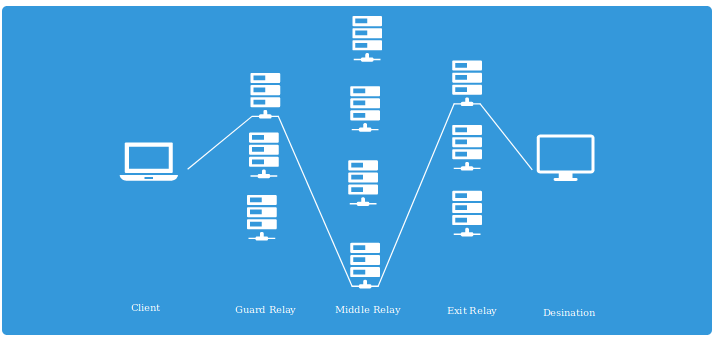
\includegraphics[scale=0.5]{fig/3relays.png}
  \caption{Cele 3 relee standard (\cite{jw1})}
  \label{fig:3rel}
\end{figure}

\begin{itemize}
  \item \textit{Releul de intrare} (eng.\ \texttt{entry/guard}), prin care conexiunea
    intră în rețeaua Tor. Asemenea relee sînt alese după ce au dovedit o vechime
    în rețea, stabilitate și lățime de bandă corespunzătoare.
  \item \emph{Relee intermediare} sînt cele care transmit conexiunea mai departe.
    Totodată, în ideea anonimizării, rolul lor este ca releele de intrare și cele
    de ieșire să nu se cunoască între ele.
  \item \emph{Releul de ieșire}, care se află la capătul rețelei Tor și trimit 
    traficul către destinația finală dorită de client.
\end{itemize}
\index{releu}
\index{releu!de intrare}
\index{releu!intermediar}
\index{releu!de ieșire}

De remarcat este faptul că, dacă releele intermediare pot fi orice calculator, server
etc., care nu se compromit în niciun fel, deoarece ele nu fac decît să transporte
trafic deja criptat, releele de ieșire au o responsabilitate deosebită. În cazul unei
conexiuni ilicite, traficul către destinație apare ca fiind transmis de la releul
de ieșire, ceea ce-i expune în mod deosebit.

La fiecare pas se realizează o decriptare, dacă traficul circulă de la client către
server și o criptare, dacă traficul circulă invers. Așa cum am menționat în secțiunea
anterioară, fiecare nod intermediar adaugă sau elimină cîte un strat criptografic,
realizînd \qq{rutarea în foi de ceapă}.

\begin{figure}[!htbp]
  \centering
  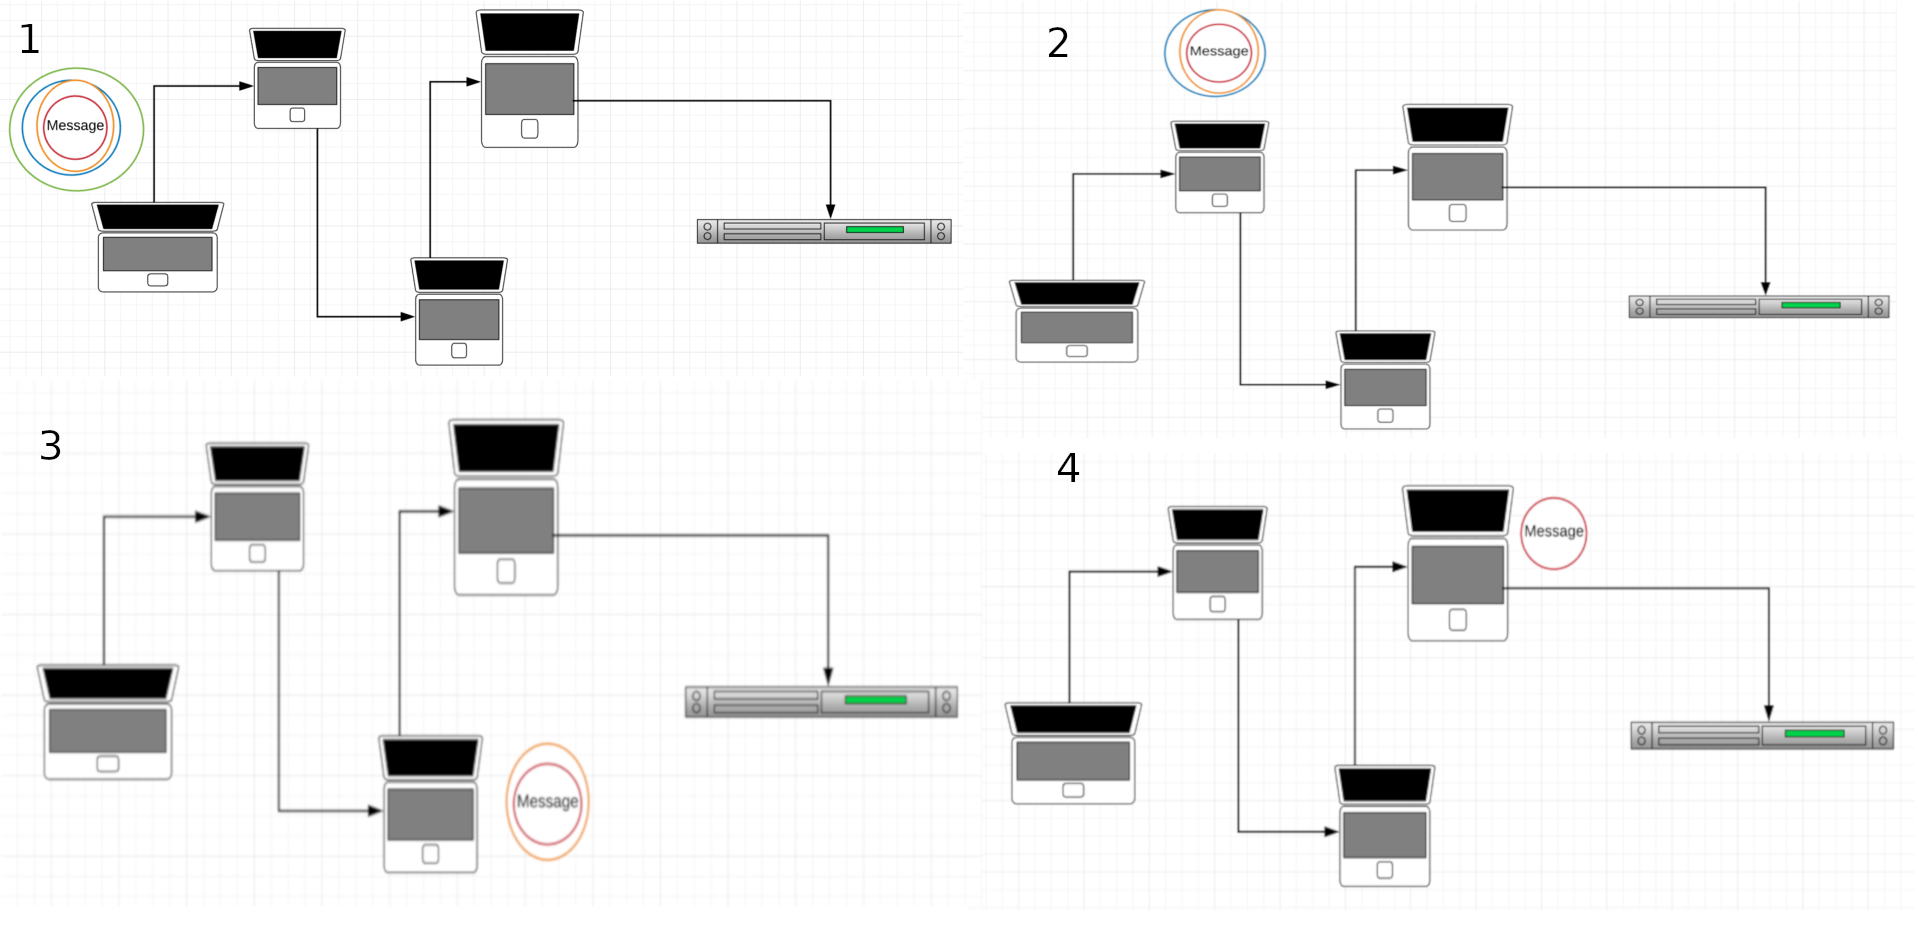
\includegraphics{fig/4onions.png}
  \caption{\qq{Foile de ceapă} (\cite{bs})}
  \label{fig:4on}
\end{figure}


Prin acest mecanism, fiecare releu cunoaște doar minimul necesar: nodul anterior și
nodul care va urma, realizînd \emph{criptarea telescopică} despre care am mai vorbit.
De remarcat este faptul că releul de ieșire vede datele inițiale trimise de client.
Astfel, dacă se trimit date sensibile prin protocoale care folosesc text clar, precum
HTTP sau FTP, releul de ieșire poate să intercepteze traficul.

%%%%%%%%%%%%%%%%%%%%%%%%%%%%%%%%%%%%%%%%%%%%%%%%%%%%%%%%%%%%%%%%%%%%%%

\section{Poduri} \index{poduri}

\indent\indent Utilizarea releelor, în forma descrisă mai sus, ridică o vulnerabilitate
serioasă. Astfel, atunci cînd un client se conectează la rețea, trebuie să aibă acces
la lista tuturor releelor de intrare, mediane și de ieșire, pentru a ști unde s-ar putea
conecta. Lista releelor nu este secretă, ceea ce ridică o potențială problemă de securitate.

O soluție pentru această problemă este utilizarea \emph{podurilor} (eng.\ \texttt{bridges}).
Într-o formă simplificată, putem privi podurile ca intrări secrete în relee, pe care le
pot accesa, de exemplu, utilizatori care se află în spatele unor rețele cenzurate.

Există și o listă completă de poduri, deținută de proiectul Tor, dar această listă
nu este publicată. Cei de la Tor au găsit o soluție prin care utilizatorii să aibă
acces doar la o porțiune mică a listei podurilor, suficiente pentru a iniția o conexiune.
Astfel, utilizatorul nici nu are nevoie de toate podurile disponibile, ci doar de cîteva
pentru a-și face intrarea în rețea.

Cercetătorii au reușit să identifice între 79\% și 86\% din lista totală a podurilor,
realizînd o analiză a întregului spațiu de adrese IPv4, dar chiar și așa, putem considera
că secretul listei podurilor este suficient de bine păstrat.

%%%%%%%%%%%%%%%%%%%%%%%%%%%%%%%%%%%%%%%%%%%%%%%%%%%%%%%%%%%%%%%%%%%%%%
\section{Autorități directoare} \index{autorități directoare}

\indent\indent Am menționat în prima parte faptul că în rețea există o serie
de autorități directoare, care sînt nodurile cele mai de încredere și, într-un fel,
țin funcționare proiectului în spate.

Statusul releelor Tor este ținut într-un document dinamic, numit \emph{consens}. \index{consens}
Acest document este întreținut de autoritățile directoare (AD) și actualizat
în fiecare oră prin voturi, în următorul mod:
\begin{itemize}
  \item fiecare AD face o listă de relee cunoscute;
  \item fiecare AD calculează și ceilalți parametri necesari despre relee (țara,
    lățimea de bandă etc.);
  \item AD transmite această informație sub forma unui status celorlalte AD;
  \item fiecare AD primește acest status, din care își actualizează propria
    listă;
  \item toți parametrii adunați de la toate AD sînt combinate și se calculează
    un vot, care este transmis cu o semnătură de către fiecare AD;
  \item releele care primesc majoritatea voturilor sînt păstrate în consens, care
    se actualizează și se transmite tuturor AD.
\end{itemize}

Procesul de vot și actualizare de mai sus este public, transmis prin HTTP, astfel
încît poate fi accesat de orice utilizator.

%! TEX root = ../tor.tex

\chapter{Atacuri și strategii de apărare}

\indent\indent În lucrarea inițială de prezentare a tehnologiei Tor (\cite{whitepaper}),
apar diverse tipuri de atacuri pe care cercetătorii le prevăzuseră, împreună cu
modurile de apărare.

\section{Atacuri pasive}

\indent\indent Un atac pasiv clasic este reprezentat de \emph{observarea tiparelor %
din traficul utilizatorilor}. Astfel, deși identitatea utilizatorilor rămîne
necunoscută, se poate profila traficul și găsi diverse tipare în modul lor
de utilizare. Totuși, sarcina este îngreunată de faptul că pot circula mai
multe fire prin același circuit, așa cum am menționat în prima parte a lucrării,
deci conexiunile interceptate pot să nu aparțină utilizatorului-țintă.

Un alt tip de atac tipic este dat de \emph{observarea conținutului utilizatorului}.
Deși la nivelul utilizatorului, conținutul este criptat, conexiunile către
serverele care trimit răspunsul, pot să nu fie (de exemplu, conexiunea de
la releul final la serverul adresat). Se poate chiar ca serverul accesat să
fie ostil și să încerce să atace utilizatorul. Tor nu urmărește să filtreze
conținutul, dar se poate apăra împotriva acestui atac folosind servicii terțe
precum Privoxy sau altele similare pentru filtrare.

Faptul că este permis fiecărui utilizator să-și configureze conexiunea poate
fi o vulnerabilitate. De exemplu, utilizatorii mai avansați sau cei care
ar avea nevoie de anonimitate sau intimitate mai pronunțată, pot cere schimbarea
circuitului foarte des. Dar aceasta poate fi o vulnerabilitate pentru utilizatorii
\qq{normali}, deoarece îi evidențiază ca pe o posibilă minoritate.

Așa cum am mai menționat, un alt atac clasic poate fi \emph{corelația la ambele capete}.
Un observator global ar putea să identifice și să profileze mai bine traficul,
dar în realitate, acest atac este aproape imposibil. Mai mult decît atît,
cum Tor folosește topologia țevii cu scurgeri, se poate întîmpla ca un utilizator
să ceară ieșirea din rețea înainte de capăt, iar atunci observatorul, chiar cu
puteri globale, este compromis.

\index{atac!de confirmare}
\index{atac!website fingerprinting}
\index{atac!de corelație}
Atacurile de mai sus se încadrează în categoria \emph{atacurilor de confirmare}.
Prin observarea traficului, se poate confirma că s-a realizat o anumită
conexiune de interes. Dar există și un alt atac cu potențial mai periculos,
de care Tor nu poate apăra foarte eficient: \emph{amprentarea site-urilor}
(eng.\ \texttt{website fingerprinting}). În locul căutării conexiunilor de
intrare sau ieșire pentru profilare, atacatorul poate să-și facă o bază
de date de \qq{amprente} care conțin tipare de acces și mărimi de fișiere
schimbate de client cu site-uri țintă. În cazul Tor, eficiența acestui
atac nu este foarte mare, deoarece se folosesc mai multe fire în format
multiplex prin aceeași rețea și mai mult, amprentele sînt limitate de
mărimea celulelor de trafic, adică de 512 octeți. Sugestii pentru îmbunătățirea
securității din acest punct de vedere ar fi să se utilizeze scheme de grupare
a traficului către anumite site-uri sau padding aplicat link-urilor.


%%%%%%%%%%%%%%%%%%%%%%%%%%%%%%%%%%%%%%%%%%%%%%%%%%%%%%%%%%%%%%%%%%%%%%
\section{Atacuri active}

\indent\indent Un atacator care află cheia de sesiune TLS ar putea
să controleze celulele și releele din circuit. Totodată, aflarea
acestei chei îi permite să desfacă un strat din criptare și, dacă
află cheia unui OR, poate să \qq{devină} acel OR pe durata vieții
cheii. Însă atacul nu este foarte util, deoarece, pentru a putea crea
într-adevăr impresia că este acel OR, trebuie să aibă acces și la cheia
onion pentru a decripta celulele \texttt{create}. Dar, cum conexiunea
are securitate perfectă la înaintare, de îndată ce s-a făcut o legătură
în rețea, ea nu mai poate fi compromisă. Totodată, rotația cheilor
limitează perioada în care asemenea atacuri pot acționa. Astfel că,
în realitate, un asemenea atac poate fi eficient doar dacă se poate
lansa pe durata vieții unei conexiuni. Situația este puțin probabilă,
dar pot exista cazuri legale sau extralegale cînd autorități de un
anume rang pot cere accesul la anumite noduri. A fost cazul în 2003,
cînd autoritățile germane au obținut un mandat de spargere a protocoalelor
serviciului de anonimizare \texttt{Java Anon Proxy} (\cite{jap}).

În plus, dacă atacatorul află cheia de identitate a unui nod, poate
contacta serverele directoare și să trimită descrieri false, infiltrîndu-se
în aceste servere.
\index{atac!compromiterea cheilor}

Un alt tip de atac activ care poate fi lansat este prin rularea unui server.
Dacă un atacator creează un server web care să ofere conținut prin care
să atragă utilizatori ai rețelei Tor, atunci el are șanse să intre în rețea
și să fie accesat de noduri de ieșire. În acest caz, poate afla diverse
tipare de trafic sau poate trimite conținut malițios, deoarece are control
asupra unui capăt al conexiunii. Similar este și cazul cînd un atacator
deține un OR ostil. Dar, dacă atacatorul deține controlul asupra $ m > 1 $
din $ N $ noduri, se poate arăta că el poate corela cel mult $ \Big(\dfrac{m}{n}\Big)^2 $
din trafic, conform \cite{bs}. Acest număr, deși poate fi neglijabil 
(amintim că $ N > 6000 $), poate fi grupat cu alte atacuri, precum acela 
al rulării unui server care să atragă trafic.

În ce privește atacurile asupra celulelor, amintim că la fiecare nod se
fac verificări de integritate, deci acestea nu pot fi atacate cu succes.

În cazul în care utilizatorul vrea să se conecteze la un server printr-un
protocol nesecurizat, precum HTTP, se poate ca un atacator să se dea drept
serverul-țintă. De aceea, utilizatorii se pot proteja de o asemenea situație
conectîndu-se cu protocoale care fac autentificarea la ambele capete.

Desigur, alte tipuri de atacuri care țin de faptul că rețeaua este menținută
activă de voluntari pot fi distribuirea de cod ostil din partea unui utilizator
de încredere sau acțiuni interzise din punctul de vedere al politicilor
de ieșire sau de rutare ori din punct de vedere social.

%%%%%%%%%%%%%%%%%%%%%%%%%%%%%%%%%%%%%%%%%%%%%%%%%%%%%%%%%%%%%%%%%%%%%%

\section{Atacuri asupra directoarelor}

\index{atac!pe directoare}
\indent\indent În cazul în care se distrug servere directoare, rețeaua
este proiectată pentru a continua să funcționeze, deoarece încă se
primesc semnături și voturi în consens din partea serverelor încă
active. Însă, din design, dacă se distrug peste jumătate din serverele
directoare, este necesară intervenția umană, deoarece consensul nu mai
are suficiente date.

Atacul asupra unei singure autorități directoare, însă, nu este tocmai
eficient, deoarece consensul înregistrează voturi, iar acest atac ar
putea, în cel mai rău caz (dar total nepractic) să influențeze aceste
voturi, înclinînd balanța către autorizarea unor servere ostile.
În practică, asemenea atacuri nu au apărut, deci nu există precedențe
pentru a se face analize de impact.

Și în aceste cazuri, pot apărea atacuri datorate naturii umane. De exemplu,
se poate păcăli o autoritate directoare că un OR funcționează, deși este
stricat sau că este valid, deși este malițios sau convingerea pentru listarea unui
server drept autoritate directoare. Tor nu apără împotriva unor asemenea
atacuri.

%%%%%%%%%%%%%%%%%%%%%%%%%%%%%%%%%%%%%%%%%%%%%%%%%%%%%%%%%%%%%%%%%%%%%%

\section{Cenzură și atacuri politice}
\index{atac!cenzură}
\indent\indent Un atac special, care poate fi lansat de un atacator
ostil sau comandat politic (sub formă de cenzură, de exemplu), ar putea
să vizeze traficul care intră sau care iese din Tor, adică să împiedice
utilizatorii să intre în rețea sau să iasă către destinație.

Blocarea nodurilor de ieșire este o situație care poate avea loc, deoarece
lista nodurilor de ieșire este publică, iar Tor nu se poate apăra de
asemenea atacuri. Un atacator poate pur și simplu să dezactiveze nodul
de ieșire sau să-l inunde cu cereri, lucru care l-ar face inutilizabil.

În celălalt caz, însă, blocarea nodurilor de intrare este imposibilă,
mulțumită podurilor. Aceasta deoarece lista tuturor nodurilor de intrare 
nu este disponibilă, iar lista podurilor poate fi descoperită doar parțial.
Se poate, cel mult, combina acest tip de atac cu cel de corelarea traficului.
Dacă atacatorul are date acumulate despre anumiți utilizatori, despre care
se crede că se conectează la anumite noduri de intrare (sau acest lucru este
surprins în timp ce se întîmplă), se pot lansa atacuri asupra acelui nod.
Atacurile de tip \qq{inundație} (eng.\ \texttt{flood}) sînt cele mai ușoare
și ar putea dezactiva nodul de intrare.


%! TEX root = ../tor.tex

\chapter{Tor vs VPN}


%%%%%%%%%%%%%%%%%%%%%%%%%%%%%%%%%%%%%%%%%%%%%%%%%%%%%%%%%%%%%%%%%%%%%%
% INDEX
\renewcommand{\indexname}{Index}
\addcontentsline{toc}{chapter}{\protect\numberline{}Index}
\printindex

% BIBLIOGRAFIE
\bibliography{tor.bib}
\bibliographystyle{apalike}
\nocite{*}
\addcontentsline{toc}{chapter}{\protect\numberline{}Bibliografie}

\end{document}
